% For help on subfiles see https://www.sharelatex.com/learn/Multi-file_LaTeX_projects
\documentclass[../main.tex]{subfile}
\begin{document}
	
		\todo[inline]{Add info from tutorials on http://www.fasteque.com/android-reverse-engineering-101-part-5/}
		\paragraph{} There are several static analysis tools available for APKs, each one having its own strengths and weaknesses. We will be using androguard because of it can be easily automated to analyze large amount of applications and store the result in a database. Other popular static analysis tools include Smali/Backsmali, apktool, JADX-Dex to java decompiler, Dex2Jar, Jd-gui etc.
		%\todo[inline]{Add info about similarity search to identify malwares or relation between them}
		%\todo[inline]{Add info from http://orbilu.uni.lu/bitstream/10993/26879/1/tr\textunderscore slr\textunderscore article.pdf}
		%\todo[inline]{Add some info about common tools}
		%\subsection{Smali/Backsmali}
		%\paragraph{} smali/backsmali is an assembler/disassembler for the dex format. More detailed information can be found on its github repository \cite{smali/backsmali_github}.
		%\subsection{IDA pro}
		%\subsection{JADX - Dex to Java decompiler}
		% https://github.com/skylot/jadx
		%\subsection{Apktool}\label{sec:apktool}
		%APKTool is one of the major reverse engineering tools for android applications.  \todo[inline]{Add more %info}
		%\subsection{Dex2Jar and jd-gui}
		% dex2jar : https://sourceforge.net/projects/dex2jar/
		% jd-gui : http://jd.benow.ca/
		
		\subsection{Androguard}\label{sec:androguard}
		\todo[inline]{Introduce androguard}
		\todo[inline]{MalloDroid, extension of androguard https://www.dfn-cert.de/dokumente/workshop/2013/FolienSmith.pdf}
		\todo[inline]{Androguard used in http://lilicoding.github.io/SA3Repo/papers/2013\textunderscore guo2013characterizing.pdf}
		\paragraph{} Androguard is an open source tool written in python for analyzing android applications. Its been used in several tools including Virustotal and Cuckoodroid among others. It can process APK files, dex files or odex files. It can disassemble Dex/Odex files to smali code and can decompile Dex/Odex to Java code. Being python based and open source it allows for automating most the analysis process and one can make desired improvements.
		
		\paragraph{} Androguard doesn't have a lot of documentation available online and most of the time one has to figure it out from source code of androguard. For easier understanding and use, we can generalize the classes androgaurd contain into two groups as shown in table \ref{table:androguard_classes}.
				
		\begin{table} \todo[inline]{Fix the position of table}
			\begin{center}
				\begin{tabular}{|p{5cm}|p{5cm}|}
					\hline \textbf{Classes for Parsing} & \textbf{Classes for Analysis}\\ \hline
					\begin{itemize}
						\item \textbf{APK} Used for accessing all elements inside an APK, including information from Manifest.xml like permissions, activities etc.
						\item \textbf{DalvikVMFormat}	It parses the dex file and gives access classes, methods, strings etc. defined inside the dex file.
						\item \textbf{ClassDefItem} Class for interacting with class information inside the dex file.
						\item \textbf{EncodedMethod} Class for interacting with method information inside the dex file. 
						\item \textbf{Instuction} Class for interacting with instructions, it contains mnem, opcodes etc. Its a base class and a androguard derive a class for each instruction format from this class.
					\end{itemize}
					
					&
					
					\begin{itemize}
						\item \textbf{Analysis} Its the main analysis class and contain instances of all other analysis classes discussed below. create\textunderscore xref() method needs to be called after an instance of this class is created to populate all defined fields in this class.
						\item \textbf{ClassAnalysis} This class contain analysis data of a class like cross references and external methods etc.
						\item \textbf{MethodAnalysis} Contain analysis information of a method like the basic blocks it is composed of etc.
						\item \textbf{DvmBasicBlock} Represents a simple basic block of a method. It contains information about that basic block like its parents, children etc.
						\end{itemize}\\ \hline
					
				\end{tabular}
			\end{center}
			\caption{Some classes of androguard and their description}
			\label{table:androguard_classes}
		\end{table}
		
		\subsubsection{Androguard usage example}
				\todo[inline]{Add androguard demos}
		
		\subsubsection{Information Extracted from an APK using Androguard}
		\paragraph{} Before getting into details, we would like to mention that the information we extract will be stored in a database and similarity search would be performed on this data to figure out its relations other malware or goodware samples. The more information we have about an APK, more relations we can figure out.
		\paragraph{} Now coming towards, the extracted information, we divide it into different groups as shown in figure \ref{fig:info_extracted}.
		
		\begin{figure}
			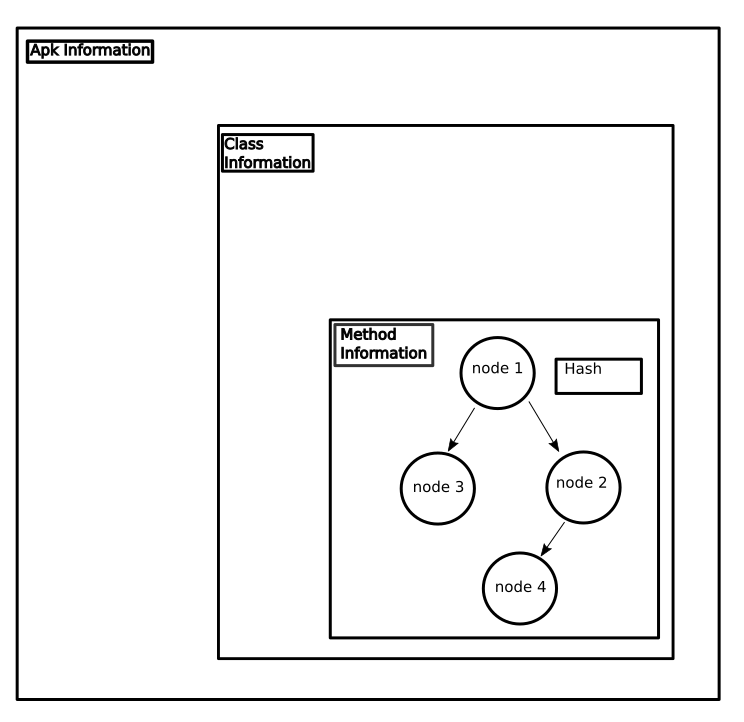
\includegraphics[width=\textwidth]{information_extracted.png}
			\caption{Groups of information extracted using APK}
			\label{fig:info_extracted}
		\end{figure}
		
		
		\begin{itemize}
			\item \textbf{APK information} This contain general information about the APK like Permissions, Package name, Libraries, Certificates, components (activities,services, receivers) and information about all classes contained in this APK.
			\item \textbf{Class information} It represent a single element of the class\textunderscore dictionary contained in APK information. It contains information like fields in the class, its access flags, name, superclass name, number of internal methods, inherited methods etc. It also contain information about methods which are part of this class in the form of a list.
			\item \textbf{Method information} A we said above, class\textunderscore information contain a list of methods\textunderscore info. Each element of that list contain information about a method such as method name, class name, address, method descriptor, length of method, its cross references, shorty descriptor, Java decompiled source code for that method, Control flow graph of that method and the calculated hash for this method.
			\item \textbf{Control Flow Graph} Control flow graph contain edges and nodes. Nodes are basic blocks and are basically a list of instructions.
			\item \textbf{Hash} Using the control flow graph a canonical hash for is computed for each method. Before computing this hash, the smali instructions are normalized according to a specific criteria so that compilation specific changes are ignored like offsets etc, \todo [inline] {Ask lukas about adding information about the hash} \todo[inline]{How much details about the normalization}
		\end{itemize}
		
		\subsubsection{Example usage}
		\paragraph{}Just to make the usage of this extracted data more clear. In this example we process some of the sonicspy samples and tried to figure out how much code the share. We analyzed 16 samples \todo[inline]{Add hashes, probably redo the whole analysis} and the result is shown in figure \ref{fig:sonicspy_freq}.
		
		\begin{figure}
			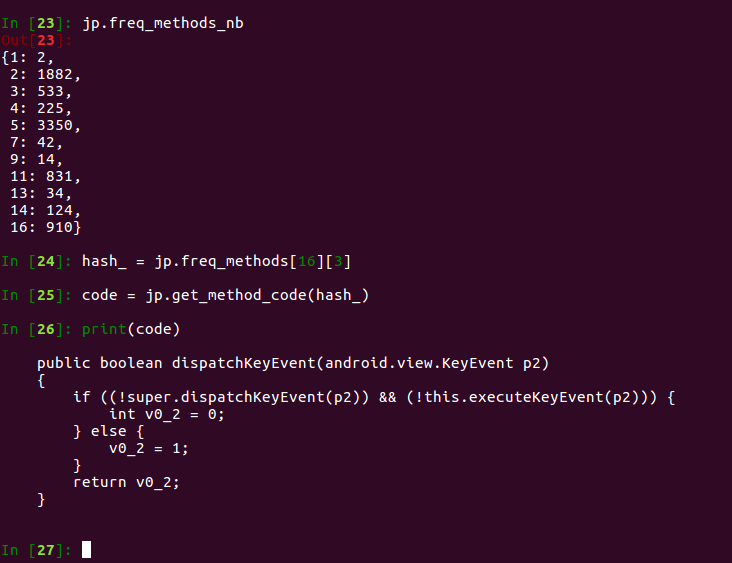
\includegraphics[width=\textwidth]{sonicspy_freq.png}
			\caption{Reused methods in sonicspy variants}
			\label{fig:sonicspy_freq}
		\end{figure}
		\paragraph{} Line 23 in figure prints the result, in this dictionary keys represent frequency or number of times a method is been reused. Value represent numbers i.e, number of methods reused a specific number of times. From this analysis we can see that a large portion of code is common between these samples but a large part of this code is not malicious. Most of it standard android API methods and non-malicious general purpose methods like wrappers etc. It would be very interesting to identify and separate API code from this chunk. It can be topic for further research to identify common non-malicious pieces of code to make analysis easier.
		
		\paragraph{} In the code snippet, "jp" is an object of a class JasonParser which we wrote just to verify information extracted from APKs. In line 24 we get the hash of a specific method and in line 25 and 26, we print its Java source code. 		
		
		\todo[inline]{TODO: Do androguard basic usage examples}
		\todo[inline]{Discuss the changes we made including normalization, canonical hasing for similarity search}
		\todo[inline]{Discuss the info we are extracting from apks for platform}
		\todo[inline]{TODO: Do androguard comparison apks to see how many functions has added and how many removed, make a table out of it}
		\todo[inline]{TODO: Find reused code section in sonicspy or bankbots or lokibot}
		\todo[inline]{Usage of androguard for extracting features for AI/ML, prepare for talk in AIOLI-FFM group}
		\todo[inline]{Ask lukas for some results from platform}
		\todo[inline]{Improvements in androguard}
\end{document}